\documentclass[onecolumn, draftclsnofoot,10pt, compsoc]{IEEEtran}
\usepackage{graphicx}
\usepackage{url}
\usepackage{setspace}
\usepackage{pdfpages}
\usepackage{geometry}
\geometry{textheight=9.5in, textwidth=7in}

% 1. Fill in these details
\def \CapstoneTeamName{		The Cleverly Named Team}
\def \CapstoneTeamNumber{		68}
\def \GroupMemberOne{			Tyler Jones}
\def \GroupMemberTwo{			Samuel Cooney}
\def \GroupMemberThree{			Aviral Sinha}
\def \CapstoneProjectName{		Investment Performance Mobile App}
\def \CapstoneSponsorCompany{	HedgeServ}
\def \CapstoneSponsorPerson{		Edison Tsai}

% 2. Uncomment the appropriate line below so that the document type works
\def \DocType{		%Problem Statement
				Requirements Document
				%Technology Review
				%Design Document
				%Progress Report
				}
			
\newcommand{\NameSigPair}[1]{\par
\makebox[2.75in][r]{#1} \hfil 	\makebox[3.25in]{\makebox[2.25in]{\hrulefill} \hfill		\makebox[.75in]{\hrulefill}}
\par\vspace{-12pt} \textit{\tiny\noindent
\makebox[2.75in]{} \hfil		\makebox[3.25in]{\makebox[2.25in][r]{Signature} \hfill	\makebox[.75in][r]{Date}}}}
% 3. If the document is not to be signed, uncomment the RENEWcommand below
%\renewcommand{\NameSigPair}[1]{#1}

%%%%%%%%%%%%%%%%%%%%%%%%%%%%%%%%%%%%%%%
\begin{document}
\begin{titlepage}
    \pagenumbering{gobble}
    \begin{singlespace}
        \hfill 
        % 4. If you have a logo, use this includegraphics command to put it on the coversheet.
        %\includegraphics[height=4cm]{CompanyLogo}   
        \par\vspace{.2in}
        \centering
        \scshape{
            \huge CS Capstone \DocType \par
            {\large\today}\par
            \vspace{.5in}
            \textbf{\Huge\CapstoneProjectName}\par
            \vfill
            {\large Prepared for}\par
            \Huge \CapstoneSponsorCompany\par
            \vspace{5pt}
            {\Large\NameSigPair{\CapstoneSponsorPerson}\par}
            {\large Prepared by }\par
            Group\CapstoneTeamNumber\par
            % 5. comment out the line below this one if you do not wish to name your team
            \CapstoneTeamName\par 
            \vspace{5pt}
            {\Large
                \NameSigPair{\GroupMemberOne}\par
                \NameSigPair{\GroupMemberTwo}\par
                \NameSigPair{\GroupMemberThree}\par
            }
            \vspace{20pt}
        }
    \end{singlespace}
\end{titlepage}
\newpage
\pagenumbering{arabic}
\tableofcontents
% 7. uncomment this (if applicable). Consider adding a page break.
%\listoffigures
%\listoftables
\clearpage

% 8. now you write!
\section{Introduction}

\subsection{Purpose}
The purpose of this mobile application will be to provide it's users insight into the quality of their investments from a portfolio level. By using this application, a user will be able to track and gain valuable insight that wouldn't be possible otherwise.

\subsection{Scope}
The scope of this project is to provide users with a method to track investments of a variety of different asset classes. Users will be able to either add investments in bulk or one investment at a time through the user interface. Upon entering an investment, the user will have a variety of options at their disposal to learn more about the quality of their investment.

\subsection{Definitions, acronyms, and abbreviations}
\begin{itemize}
	\item HedgeServ: A global, independent fund administration provider headquartered in New York with
		10 offices and 195+ clients worldwide.
	\item Xamarin: A tool built into Microsoft Visual Studio that allows developers to deliver native 
	   	C\# applications to Android, iOS, and Windows devices.
	\item C\#: (pronounced as \textit{see sharp}) is a programming language developed by Microsoft. It encompasses strong typing, imperative, declarative, functional, generic,
		object-oriented, and component-oriented programming styles.
	\item Asset: A valuable property such as resources, estate, holdings, etc...
	\item Investments: An asset or item puchased with the hope that it will geenerate income and is not consumed today and used to create wealth in the future.
	\item Portfolio: A group of financial assets that are held by investors or managed by financial professionals.
	\item Options: Contracts that grant the right but not obligation to buy or sell an underlying asset at a set price before a certain date.
	\item Currency: Money in any form that is in actual use or circulation as a medium of exchange
	\item Front End: The view of an application that provides the end user with a friendly interface to interact with.
	\item Back End: The behind the scenes of an application that typically handles business logic and the storage of data.
	\item Domain-Specific Lanuage: (Often refered to as \textit{DSL}) A programming language that has been specialized to a particular application domain.
	\item SQL: A domain-specific programming language used for managing data held in a database management system.
\end{itemize}

\subsection{Overview}

The Investment Performance Mobile Application will allow users to view their investment portfolio on iOS and Android devices
at a portfolio level. Users will have the ability to see their portfolio as well as drill down to any of their specific investments.


\subsection{Product perspective}

Currently, most mobile financial applications provide investment performance information on only one investment type at a time. 
This project seeks to solve the current lack of a tool that concurrently tracks a wide array of different investment assets in 
one consolidated source. In doing so, this application will allow users to place and view all of their investments in a single location 
while simultaneously recieving performace updates for each individual investment and the portfolio as a whole.

\subsection{Product Functions}
This mobile app will provide users investment performance from a portfolio level. The user will be able to enter investments, either 
in bulk or individually, and have their portfolio be displayed all together. Then users will have the ability to view different data
points about their portfolio as well as drill down into individual investments in order to get further data on a single asset.

While in the portfolio view, users will see a pie chart with their portfolio split up into percentages. 
For instance, if a user owns \$1000 worth of assets, these may be across various different asset classes. A user may have \$500 invested in the stock market, 
and \$500 in cryptocurrency. The pie chart would reflect this division. Additionally, the user will be able to retrieve benchmarks on their entire portfolio. 
The S\&P 500, for example, would provide the user with a benchmark by which they could compare the performance of their entire portfolio against. 
Moreover, the user will be able to disect the peformance of their entire portfolio based off a variety of time intervals. The user will see the aggregate 
performance of their investments over time intervals ranging from a week all the way to multiple years+. Lastly, the user will be able to see their Sharpe ratio and volatility of their portfolio. 
The user will also be able to see all of this data at an individual investment level. This means that this app should provide the user 
time data, the Sharpe ratio, volatility, and benchmarks of individual investments, when relevant/available.


\section{Specific requirements}

\begin{itemize}
	\item Front end development will be written in C\#, and SQL will be used for the backend. Various API's can be used to recieve data from internet sources. 
	\item There must be no longer than a 3 second response time on any given query to the database. If queries fail, the data should be blank or missing, 
		rather than inaccurate. Users should be able to rely on 100\% accurate pricing data, even if not 100\% up to date; inaccurate pricing is not an option. Crashing is better than showing incorrect data, however this crash rate should be low. Moreover, the crash rate will be measured as the number of crashes relative to the number of queries to the database, rather than crashes relative to unit time.
	\item Investment types, or asset classes, must not be hard coded - this means that the user must be able to enter any investment into the app, 
		even if there is no automated pricing data for it. 
	\item The app must support bulk data entry, or individual data entry - the user should be able to 
		add their whole portfolio at once, or add just one new investment. 
	\item Investments must be able to be removed from the portfolio, as the user should 
		have complete control over what they track. 
	\item All pages in the app should require no more than 2 taps to access from the home screen.
	\item Portfolio level will allow the user to see a pie chart of their total assets with each section being an individual investment.
	\item The portfolio will have relative benchmarks to industry standard sources like the S\&P500.
	\item An option to view the portfolio's history in a graph must be displayed with a variety of time intervals ranging from a day to weeks to multiple years.
	\item The portfolio should display the current Sharpe Ratio as well as its volatility.
	\item Individual investments should also track time data, Sharpe Ratio, Volatility, and relative benchmarks when relevant/available separate from the portfolio benchmarks.
	\item Users must be able to enter data through the application in two formats. First, one investment at a time manually added in using the user-friendly interface. Second by
		adding a CSV file or EXCEL file containing the user's portfolio data to the application will automatically populate the user's profile based off the contents of said file.
	\item Investments should list purchase price and quantity, at a minimum.
	\item Both the portfolio and individual investments should show returns based off time and purchase price.
	\item User's portfolio should be cached onto the device when the user logs in.
	\item Investment prices stored in the database should be automatically updated daily and store old data so that portfolios can track historical data.
	\item Stock splits should properlly increase investment quantity and reduce price when such event occurs (investment value should remain unchanged).
	\item The final product must be secure. Usernames and passwords must be safely stored in the database, and prevent hacking attempts such as SQL injections.
	
\end{itemize}
\section{Timeline}
Included in separate file.
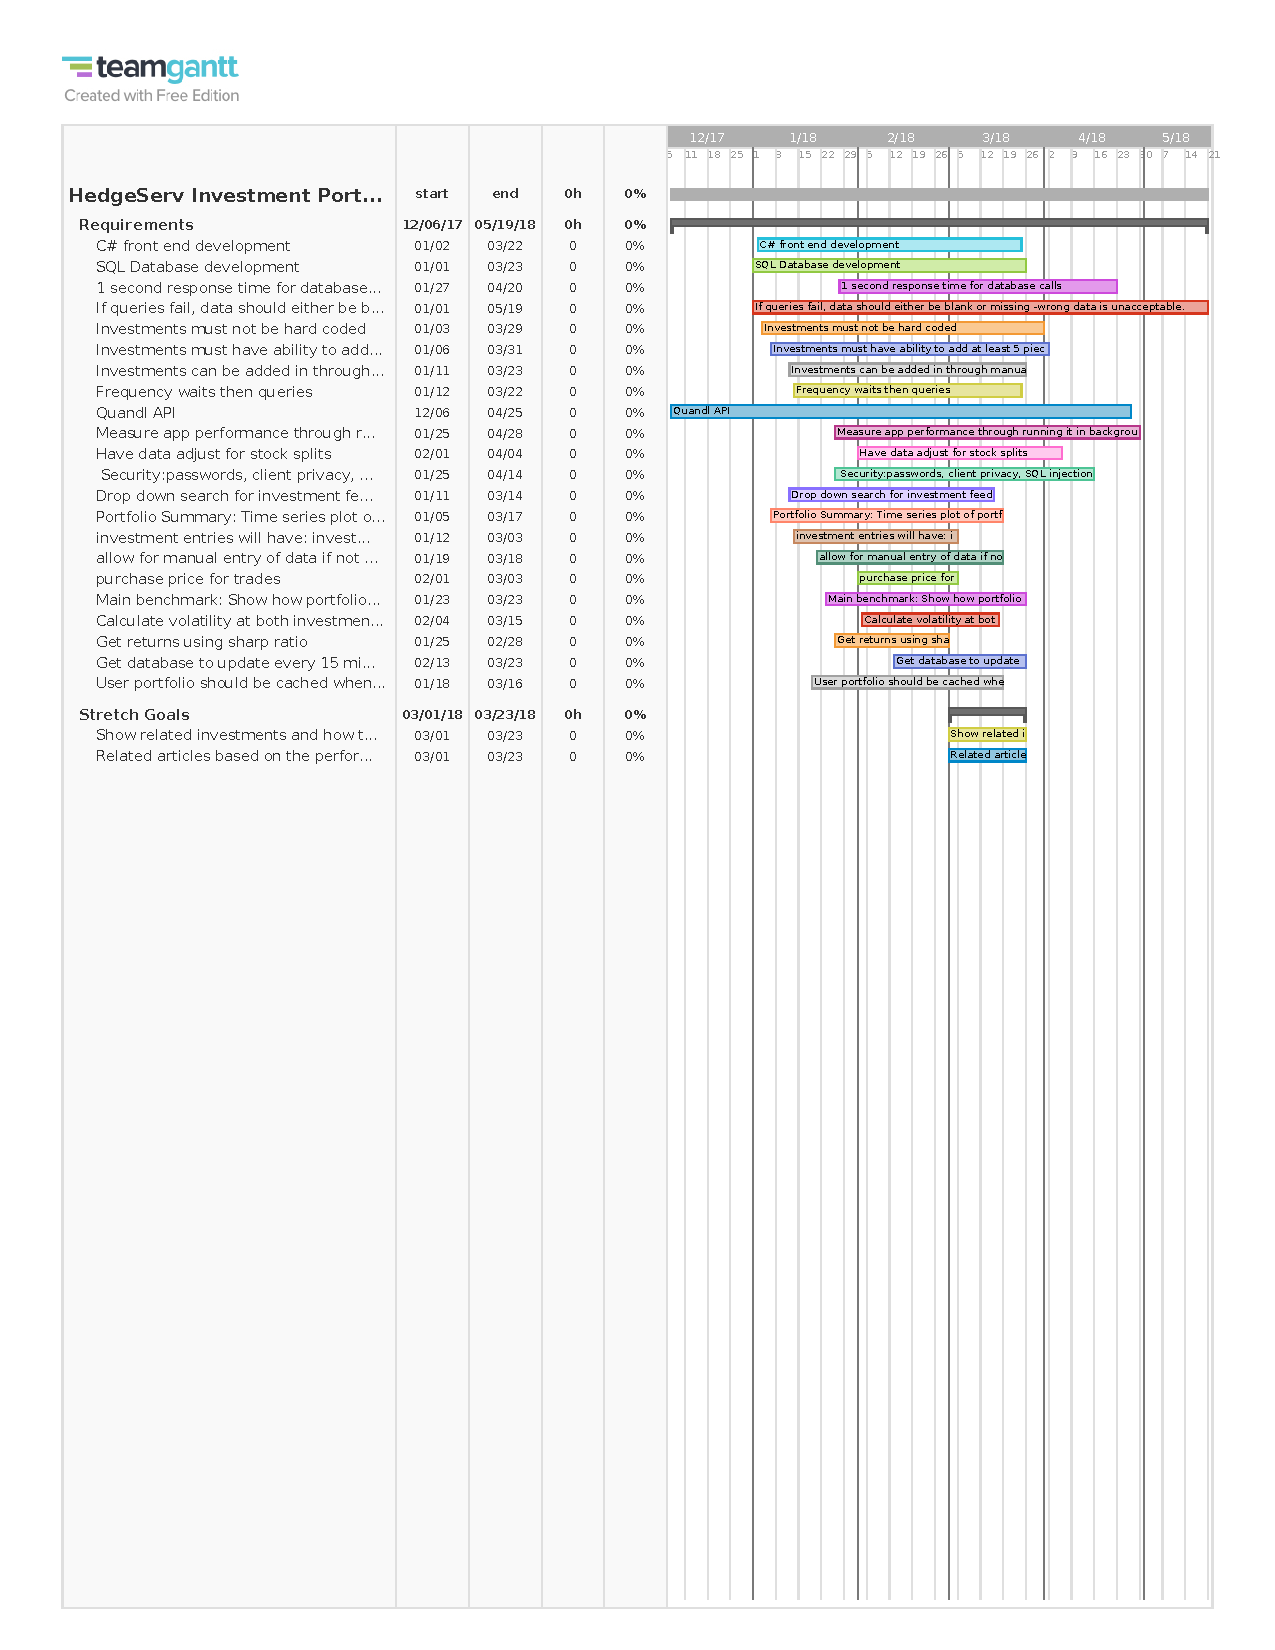
\includepdf{ganttchart.pdf}

\end{document}
